
\documentclass[a4paper,11pt]{article}
\usepackage[a4paper, margin=8em]{geometry}

% usa i pacchetti per la scrittura in italiano
\usepackage[french,italian]{babel}
\usepackage[T1]{fontenc}
\usepackage[utf8]{inputenc}
\frenchspacing 

% usa i pacchetti per la formattazione matematica
\usepackage{amsmath, amssymb, amsthm, amsfonts}

% usa altri pacchetti
\usepackage{gensymb}
\usepackage{hyperref}
\usepackage{standalone}

% imposta il titolo
\title{Appunti Calcolo Numerico}
\author{Luca Seggiani}
\date{2025}

% disegni
\usepackage{pgfplots}
\pgfplotsset{width=10cm,compat=1.9}

% imposta lo stile
% usa helvetica
\usepackage[scaled]{helvet}
% usa palatino
\usepackage{palatino}
% usa un font monospazio guardabile
\usepackage{lmodern}

% tikz in sans
\tikzset{every picture/.style={/utils/exec={\sffamily}}}

\renewcommand{\rmdefault}{ppl}
\renewcommand{\sfdefault}{phv}
\renewcommand{\ttdefault}{lmtt}

% circuiti
\usepackage{circuitikz}
\usetikzlibrary{babel}

% disponi il titolo
\makeatletter
\renewcommand{\maketitle} {
	\begin{center} 
		\begin{minipage}[t]{.8\textwidth}
			\textsf{\huge\bfseries \@title} 
		\end{minipage}%
		\begin{minipage}[t]{.2\textwidth}
			\raggedleft \vspace{-1.65em}
			\textsf{\small \@author} \vfill
			\textsf{\small \@date}
		\end{minipage}
		\par
	\end{center}

	\thispagestyle{empty}
	\pagestyle{fancy}
}
\makeatother

% disponi teoremi
\usepackage{tcolorbox}
\newtcolorbox[auto counter, number within=section]{theorem}[2][]{%
	colback=blue!10, 
	colframe=blue!40!black, 
	sharp corners=northwest,
	fonttitle=\sffamily\bfseries, 
	title=Teorema~\thetcbcounter: #2, 
	#1
}

% disponi definizioni
\newtcolorbox[auto counter, number within=section]{definition}[2][]{%
	colback=red!10,
	colframe=red!40!black,
	sharp corners=northwest,
	fonttitle=\sffamily\bfseries,
	title=Definizione~\thetcbcounter: #2,
	#1
}

% disponi problemi
\newtcolorbox[auto counter, number within=section]{problem}[2][]{%
	colback=green!10,
	colframe=green!40!black,
	sharp corners=northwest,
	fonttitle=\sffamily\bfseries,
	title=Problema~\thetcbcounter: #2,
	#1
}

% disponi codice
\usepackage{listings}
\usepackage[table]{xcolor}

\definecolor{codegreen}{rgb}{0,0.6,0}
\definecolor{codegray}{rgb}{0.5,0.5,0.5}
\definecolor{codepurple}{rgb}{0.58,0,0.82}
\definecolor{backcolour}{rgb}{0.95,0.95,0.92}

\lstdefinestyle{codestyle}{
		backgroundcolor=\color{black!5}, 
		commentstyle=\color{codegreen},
		keywordstyle=\bfseries\color{magenta},
		numberstyle=\sffamily\tiny\color{black!60},
		stringstyle=\color{green!50!black},
		basicstyle=\ttfamily\footnotesize,
		breakatwhitespace=false,         
		breaklines=true,                 
		captionpos=b,                    
		keepspaces=true,                 
		numbers=left,                    
		numbersep=5pt,                  
		showspaces=false,                
		showstringspaces=false,
		showtabs=false,                  
		tabsize=2
}

\lstdefinestyle{shellstyle}{
		backgroundcolor=\color{black!5}, 
		basicstyle=\ttfamily\footnotesize\color{black}, 
		commentstyle=\color{black}, 
		keywordstyle=\color{black},
		numberstyle=\color{black!5},
		stringstyle=\color{black}, 
		showspaces=false,
		showstringspaces=false, 
		showtabs=false, 
		tabsize=2, 
		numbers=none, 
		breaklines=true
}

\lstdefinelanguage{javascript}{
	keywords={typeof, new, true, false, catch, function, return, null, catch, switch, var, if, in, while, do, else, case, break},
	keywordstyle=\color{blue}\bfseries,
	ndkeywords={class, export, boolean, throw, implements, import, this},
	ndkeywordstyle=\color{darkgray}\bfseries,
	identifierstyle=\color{black},
	sensitive=false,
	comment=[l]{//},
	morecomment=[s]{/*}{*/},
	commentstyle=\color{purple}\ttfamily,
	stringstyle=\color{red}\ttfamily,
	morestring=[b]',
	morestring=[b]"
}

% disponi sezioni
\usepackage{titlesec}

\titleformat{\section}
	{\sffamily\Large\bfseries} 
	{\thesection}{1em}{} 
\titleformat{\subsection}
	{\sffamily\large\bfseries}   
	{\thesubsection}{1em}{} 
\titleformat{\subsubsection}
	{\sffamily\normalsize\bfseries} 
	{\thesubsubsection}{1em}{}

% disponi alberi
\usepackage{forest}

\forestset{
	rectstyle/.style={
		for tree={rectangle,draw,font=\large\sffamily}
	},
	roundstyle/.style={
		for tree={circle,draw,font=\large}
	}
}

% disponi algoritmi
\usepackage{algorithm}
\usepackage{algorithmic}
\makeatletter
\renewcommand{\ALG@name}{Algoritmo}
\makeatother

% disponi numeri di pagina
\usepackage{fancyhdr}
\fancyhf{} 
\fancyfoot[L]{\sffamily{\thepage}}

\makeatletter
\fancyhead[L]{\raisebox{1ex}[0pt][0pt]{\sffamily{\@title \ \@date}}} 
\fancyhead[R]{\raisebox{1ex}[0pt][0pt]{\sffamily{\@author}}}
\makeatother

\begin{document}

% sezione (data)
\section{Lezione del 07-04-25}

% stili pagina
\thispagestyle{empty}
\pagestyle{fancy}

% testo
\subsection{Interpolazione di funzioni}
Poniamo di avere una qualche funzione $f(x) : \mathbb{C} \rightarrow \mathbb{C}$ (in realtà spesso prenderemo senza ledere alla generalità della trattazione $f(x) : \mathbb{R} \rightarrow \mathbb{R}$) che non conosciamo esplicitamente ma di cui possiamo solo calcolare il valore $y_0, ..., y_k$ in determinati punti $x_0, ..., x_k$ non necessariamente equspaziati fra di loro.
Chiamiamo questi punti \textbf{nodi}.
Il problema sarà allora trovare un'\textit{approssimazione} di $f(x)$ \textbf{interpolando} i punti dati.
\begin{itemize}
	\item 
Un approccio valido quando si hanno pochi punti ($k$) è considerare un polinomio di grado $k$ che passi per tutti questi, sperando che si raggiunga un'approssimazione sufficientemente precisa nei punti esterni ai nodi.
Questo è l'approccio che vedremo della sezione 13.1.1 in poi;
	\item
Un altro approccio, quando si hanno molti punti, è trovare una funzione particolarmente semplice (solitamente una retta) che minimizzi la distanza da questi.
E' questo ad esempio il caso della \textit{regressione lineare}.
Questo è l'approccio dell'\textit{approssimazione ai minimi quadrati} che vedremo in 15.2.
\end{itemize}

\subsubsection{Interpolazione polinomiale}
Vogliamo quindi trovare un polinomio $p(x)$ tale che:
$$
p(x_i) = y_i, \quad \forall i \in \{ 0, ..., k \}
$$
Quello che facciamo è porre il polinomio come:
$$
p(x) = a_0 + a_1 x + ... a_k x^k
$$
e impostare il sistema:
\[
	\begin{cases}
		a_0 + a_1 x_0 + ... + a_k x_0^k = y_0 \\ 
		\vdots \\
		a_0 + a_1 x_k + ... + a_k x_k^k = y_k
	\end{cases}
\]
che è lineare e ha come incognita il vettore dei coefficienti del polinomio cercato.

Notiamo di aver scelto come base la base canonica dei polinomi:
$$
B_\text{canonica} = \left\{ 1, x, x^2, ..., x^k \right\}
$$
Avremmo potuto scegliere qualsiasi altra base dello spazio dei polinomi $\mathbb{R}[x]$, e vedremo infatti anche questo caso.

Riscrivendo quindi il sistema di cui sopra in forma matriciale si ha:
$$
\underbrace{
\begin{pmatrix}
	1 & x_0 & ... & x_0^k \\
	\vdots  & & & \vdots \\
	1 & x_k & ... & x_k^k \\
\end{pmatrix}
}_V
\underbrace{
\begin{pmatrix}
	a_0 \\ a_1 \\ \vdots \\ a_k
\end{pmatrix}
}_a
=
\underbrace{
\begin{pmatrix}
	y_0 \\ y_1 \\ \vdots \\ y_k 
\end{pmatrix}
}_y
$$
dove la matrice $V$ viene detta \textbf{matrice di Vandermonde}.

Potrebe interessarci capire quando questo sistema ammette soluzione.
Ad esempio, è impossibile che esista $i \neq j$ tali che $x_i = x_j$, in quanto questo renderebbe il sistema singolare (due righe uguali $\implies \det(V) = 0$).
Questo caso non è desiderabile in quanto potrebbero esserci più soluzioni (se anche $y_i = y_j$) o nessuna (se $y_i \neq y_j$).

Possiamo allora enunciare il teorema:
\begin{theorem}{Determinante della matrice di Vandermonde}
	Il determinante della matrice di Vandermonde è:
	$$
	\det(V) = \prod_{0 \leq i < j \leq k} (x_j - x_i)
	$$
\end{theorem}
Possiamo dare una dimostrazione immediata di questo risultato ricordando che si può aggiungere un multiplo scalare di una colonna ad un altra colonna senza cambiare il determinante.
Prendiamo allora la matrice nella forma più completa:

$$
V = 
\begin{pmatrix}
	1 & x_0 & x_0^2 & ... & x_0^k \\
	1 & x_1 & x_1^2 & ... & x_1^k \\
	1 & x_2 & x_2^2 & ... & x_2^k \\
	\vdots & & & & \vdots \\
	1 & x_k & x_k^2 & ... & x_k^k \\
\end{pmatrix}
$$

Sottraiamo quindi ad ogni colonna dopo la prima il prodotto della colonna precedente per $x_0$, cancellando effettivamente la prima riga:

$$
\rightarrow
\begin{pmatrix}
	1 & 0 & 0 & ... & 0 \\
	1 & x_1 - x_0 & x_1^2 - x_1x_0 & ... & x_1^k - x_1^{k - 1} x_0 \\
	1 & x_2 - x_0 & x_2^2 - x_2x_0 & ... & x_2^k - x_1^{k - 1} x_0 \\
	\vdots & & & & \vdots \\
	1 & x_k - x_0 & x_k^2 - x_k x_0 & ... & x_k^k - x_1^{k - 1} x_0 \\
\end{pmatrix}
$$
$$
=
\begin{pmatrix}
	1 & 0 & 0 & ... & 0 \\
	1 & x_1 - x_0 & x_1(x_1 - x_0) & ... & x_1^{k - 1} (x_1 - x_0) \\
	1 & x_2 - x_0 & x_2(x_2 - x_0) & ... & x_2^{k - 1} (x_2 - x_0) \\
	\vdots & & & & \vdots \\
	1 & x_k - x_0 & x_k(x_k - x_0) & ... & x_k^{k - 1} (x_k - x_0) \\
\end{pmatrix}
$$

Continuiamo questo procedimento sottraendo stavolta dalla colonna 2 in poi, e moltiplicando per $x_1$:
$$
\rightarrow
\begin{pmatrix}
	1 & 0 & 0 & ... & 0 \\
	1 & x_1 - x_0 & 0  & ... & 0 \\
	1 & x_2 - x_0 & x_2(x_2 - x_0) - x_1(x_2 - x_0) & ... & x_2^{k - 1} (x_2 - x_0) - x_1 (x_2 - x_0) \\
	\vdots & & & & \vdots \\
	1 & x_k - x_0 & x_k(x_k - x_0) - x_1 (x_k - x_0) & ... & x_k^{k - 1} (x_k - x_0) - x_1 (x_k - x_0) \\
\end{pmatrix}
$$
$$
=
\begin{pmatrix}
	1 & 0 & 0 & ... & 0 \\
	1 & x_1 - x_0 & 0 & ... & 0 \\
	1 & x_2 - x_0 & (x_2 - x_1)(x_2 - x_0) & ... & (x_2^{k - 1} - x_1) (x_2 - x_0) \\
	\vdots & & & & \vdots \\
	1 & x_k - x_0 & (x_k - x_1) (x_k - x_0) & ... & (x_k^{k - 1} - x_1) (x_k - x_0) \\
\end{pmatrix}
$$

Dovrebbe quindi risultare chiaro che ripetendo questa operazione $k$ volte si ottiene una matrice triangolare inferiore, di cui ricordiamo il determinante si calcola moltiplicando gli elementi sulla diagonale, cioè si ottiene:
$$
\det(V) = 1 \cdot (x_1 - x_0) \cdot (x_2 - x_1) (x_2 - x_0) \cdot ... = \prod_{0 \leq i < j \leq k} (x_j - x_i)
$$
che è (gesticolando un pò) la tesi. \qed

Da questo deriva il \textbf{corollario} immediato che se $x_i \neq x_j$ $\forall i \neq j$, allora $\det(V) \neq 0$, cioè $V$ non è singolare.

\par\smallskip

Per trovare $p(x)$ basterà quindi risolvere il sistmea:
$$
Va = y
$$
e poniamo:
$$
p(x) = \sum_{i = 0}^k a_i x^i
$$
da cui come avevamo detto si ottiene un polinomio con $\deg(p(x)) \leq k$ ($\leq$ perchè si potrebbe avere il coefficiente $a_k = 0$, e così via, cioè il grad è \text{al più} $k$).

Risolvere il sistema costa quindi, come avevamo visto, un qualcosa che è $\sim O(n^3)$, con particolare interesse al numero di condizionamento:
$$
\mu(V) = |V| \cdot |V^{-1}|
$$
che solitamente per la matrice di Vandermonde è particolarmente grande.

\par\smallskip

Ricordiamo che questo è un problema non da poco.
Infatti, avevamo che il numero di condizionamento dava un limite alla variazione del resto del sistema in funzione della perturbazione delle soluzioni, cioè presa una $\tilde{x}$ perturbata da una $x$ soluzione di $Ax = b$ si aveva:
$$
|x - \tilde{x}| \leq \mu(A) \cdot |A \tilde{x} - b|
$$

Ad esempio, preso il sistema:
$$
\underbrace{
\begin{pmatrix}
	1 & 0 \\ 
	0 & \epsilon
\end{pmatrix}
}_A
\underbrace{
\begin{pmatrix}
	1 \\ 1
\end{pmatrix}
}_x
=
\underbrace{
\begin{pmatrix}
	1 \\ \epsilon
\end{pmatrix}
}_b
$$
potremmo pensare di considerare la soluzione perturbata:
$$
\tilde{x} =
\begin{pmatrix}
	1 \\ 1 + \delta
\end{pmatrix}
$$
Avremo quindi l'\textit{errore sulla soluzione}:
$$
|x - \tilde{x}|_2 = |\delta|
$$
e l'\textit{errore sul resto}:
$$
|A \tilde{x} - b|_2 = \left| \begin{pmatrix}
	0 \\ \delta \epsilon
\end{pmatrix} \right|_2
= |\delta| \cdot \epsilon
$$
che chiaramente cresce al crescere di $\epsilon$.

Questo ci è problematico in quanto l'\textit{errore sulla soluzione} può essere considerato come l'\textbf{errore sui coefficienti} del polinomio, e l'\textit{errore sul resto} può essere considerato come l'\textbf{errore di approssimazione} della funzione, cioè:
$$
|A \tilde{x} - b| = |p(x_i) - y_i|
$$

\par\smallskip

Vediamo che in verità la situazione è sotto controllo se:
$$
\mu(A) \leq \frac{1}{u}
$$
per $u$ precisione macchina, in quanto l'errore dato dal cattivo condizionamento diventa comparabile con la precisione macchina, comunque piuttosto piccola.
Un altro caso di interesse è quello in cui i punti $x_i$ sono equispaziati sulla circonferenza unitaria sul piano di Argand-Gauss.
Vediamo che anche qui l'errore è mantenuto sotto controllo, e questo sarà infatti il caso che considereremo per la \textit{trasformata (discreta) veloce di Fourier}.

\par\medskip

Un'idea potrebbe essere quindi quella di cambiare la base dei monomi in:
$$
B' = \left\{ \phi_0(x), \phi_1(x), ..., \phi_k(x) \right\}
$$
e porre quindi:
$$
p(x) = a_0 \phi_0(x) + a_1 \phi_1(x) + ... a_k \phi_k(x)
$$
Il sistema alla sostituzione dei nodi continuerà ad essere lineare, in quanto:
$$
p(x_i) = a_0 \phi_0(x_i) + a_1 \phi_1(x_i) + ... + a_k \phi_k(x_i), \quad \forall i \in \{ 0, ..., k \}
$$
Potremo quindi impostare un altro sistema lineare:
$$
\begin{pmatrix}
	\phi_0(x_0) & \phi_1(x_0) & ... & \phi_k(x_0) \\ 
	\vdots & & & \vdots \\
	\phi_0(x_k) & \phi_1(x_k) & ... & \phi_k(x_k) \\ 
\end{pmatrix}
\begin{pmatrix}
	a_0 \\ a_1 \\ \vdots \\ a_k
\end{pmatrix}
=
\begin{pmatrix}
	y_0 \\ y_1 \\ \vdots \\ y_k
\end{pmatrix}
$$

Abbiamo quindi definito la matrice di Vandermonde "generalizzata" a:
\begin{definition}{Matrice di Vandermonde}
	La matrice di Vandermonde su una certa base polinomiale $\{\phi_0(x), ..., \phi_k(x)\}$ è definita come:
$$
V_{ij} = \phi_j(x_i), \quad \forall i, j \in \{0, 1, ..., k\}
$$
\end{definition}
Finora avevamo preso il caso della base canonica, cioè $\{1, x, ..., x^k\}$, ma nessuno ci nega di prendere altre basi.
Basi che ci saranno di particolare interesse, vedremo, sono la base di \textbf{Lagrange} e la base di \textbf{Newton}.


\subsubsection{Base di Lagrange}
Presi sempre i nostri nodi di interpolazione, decidiamo di scegliere la base guardando proprio tali nodi (anziché prenderla a priori, come avevamo fatto per Vandermonde).

Chiamiamo i polinomi di base $l_0(x), ..., l_k(x)$, con:
$$
l_i(x) = (x - x_0) ... (x - x_{i - 1}) (x - x_{i + 1}) ... (x - x_k) = \prod_{j \neq i}^n (x - x_j)
$$
cioè il prodotto dei fattori che si annullano in $x_j$ per tutti gli $j \neq i$.
Spesso poi decidiamo di normalizzare i polinomi di base, indicandoli come:
$$
l_i(x) = \frac{(x - x_0) ... (x - x_{i - 1}) (x - x_{i + 1}) ... (x - x_k)}{(x_i - x_0) ... (x_i - x_{i - 1}) (x_i - x_{i + 1}) ... (x_i - x_k)} = \prod_{j \neq i}^n \frac{x - x_j}{x_i - x_j} 
$$
Otterremo quindi la base, diversa da quella canonica:
$$
B_\text{Lagrange} = \left\{ l_0(x), l_1(x), ..., l_k(x) \right\}
$$
Proviamo quindi ad imporre le condizione, con:
$$
p(x) = a_0 l_0(x) + a_1 l_1(x) + ... + a_k l_k(x)
$$
valutando il polinomio in un punto $x_i$:
$$
p(x_i) = y_i = a_0 l_0(x_i) + ... + a_{i - 1} l_{i - 1}(x_i) + a_i l_i(x_i) + a_{i + 1} l_{i + 1}(x_i) + ... + a_k l_k(x_i)
$$
dove vediamo che, normalizzando, si conserva solo il termine in $a_i$, da cui immediatamente:
$$
a_i = y_i
$$
e:
$$
p(x) = y_0 l_0(x) + y_1 l_1(x) + ... + y_k l_k(x)
$$
Possiamo quindi costruire il polinomio interpolante senza fare nessun conto, semplicemente prendendo la combinazione lineare a coefficienti $y_i$ della base di lagrange $l_i$ costruita sui nodi.

Vediamo quindi la forma della matrice di Vandermonde:
$$
V_l =
\begin{pmatrix}
	l_0(x_0) & l_1(x_0) & ... & l_k(x_0) \\ 
	\vdots & & & \vdots \\
	l_0(x_k) & l_1(x_l) & ... & l_k(x_k)
\end{pmatrix} = 
\begin{pmatrix}
	1 & 0 & ... & 0 \\
	0 & 1 & ... & 0 \\
	... & ... & ... & ... \\
	0 & ... & 0 & 1
\end{pmatrix}
$$
da cui abbiamo la conferma: si ricava direttamente l'identità e quindi $Va = y$ diventa $I a = y \implies a = y$.

\subsubsection{Esempio: inteprolazione di Lagrange}
A scopo di esempio, vediamo l'interpolazione di Lagrange della funzione:
$$
f\left(x\right)=\cos\left(\frac{x}{3}\right)\sin\left(2x\right)\ 
$$
con nodi equispaziati presi da $-6$ a $6$, con intervallo $1$.

Calcolando la funzione attraverso un software al computer, si otterrà la tabella di nodi:
\begin{table}[H]
	\center
	\begin{tabular} { c | p{.65cm} p{.65cm} p{.65cm} p{.65cm} p{.65cm} p{.65cm} p{.65cm} p{.65cm} p{.65cm} p{.65cm} p{.65cm} p{.65cm} p{.65cm} p{.65cm} }
		$x_j$ & $-6$ & $-5$ & $-4$ & $-3$ & $-2$ & $-1$ & $0$ & $1$ & $2$ & $3$ & $4$ & $5$ & $6$ \\
		$y_j$ & $-0.22$ & $-0.05$ & $-0.23$ & $0.15$ & $0.59$ & $-0.86$ & $0$ & $0.86$ & $-0.59$ & $-0.15$ & $0.23$ & $0.05$ & $0.22$
	\end{tabular}
\end{table}

Da cui il polinomio:
$$
p_k(x) = -0.22 l_0(x) -0.05 l_1(x) -0.23 l_2(x) +0.15 l_3(x) +0.59 l_4(x) -0.86 l_5(x) +0.86 l_6(x)
$$
$$
-0.59 l_7(x) -0.15 l_8(x) + 0.23 l_9(x) + 0.05 l_{10}(x) 0.22 l_{11}(x)
$$

\par\bigskip
\noindent

\begin{minipage}{\textwidth}
Vediamo quindi un grafico che mostra tale polinomio, sovraimposto alla funzione originale e ai nodi campionati:

\begin{center}
	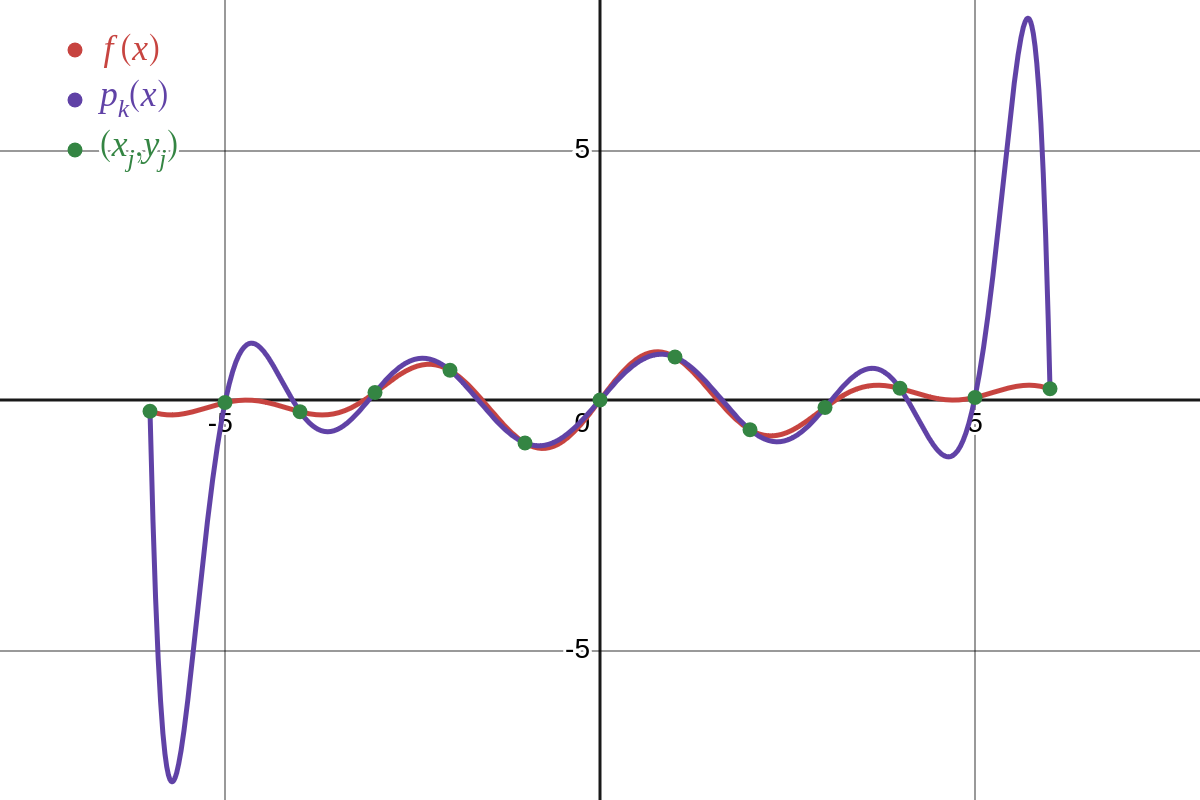
\includegraphics[scale=0.3]{../figures/lagrange_interpol.png}
\end{center}
\end{minipage}

\par\bigskip

Come vediamo, almeno nei punti intermedi l'interpolazione è piuttosto vicina, mentre ai punti estremi si notano degli artefatti non indifferente (principalmente dati dal comportamento oscillatorio della $f(x)$). 

\subsubsection{Base di Newton}
Vediamo quindi la base di Newton, che costruiamo come:
\[
	\begin{cases}
			n_0(x) = 1 \\
			n_1(x) = x - x_0 \\
			n_2(x) = (x - x_0)(x - x_1) \\
			\vdots \\
			n_k(x) = (x - x_0) ... (x - x_{k - 1})
	\end{cases}
\]
cioè ogni $n_i$ dipende solo dai $\{ x_0, ..., x_{i - 1} \}$ precedenti.
Questo rende più facile l'aggiornamento se si aggiunge un nuovo nodo in $x_{k + 1}$, per cui basterà dire:
$$
n_{k + 1}(x) = (x - x_0) ... (x - x_k) = n_k(x) (x - x_k)
$$
Otterremo quindi la base:
$$
B_\text{Newton} = \left\{ n_0(x) = 1, n_1(x), ..., n_k(x) \right\}
$$
e la matrice di Vandermonde:
$$
V_n =
\begin{pmatrix}
	n_0(x_0) & n_1(x_0) & ... & n_k(x_0) \\ 
	\vdots & & & \vdots \\
	n_0(x_k) & n_1(x_k) & ... & n_k(x_k)
\end{pmatrix}
$$
con:
$$
p(x) = a_0 n_0(x) + a_1 n_1(x) + ... + a_k n_k(x)
$$
e nel nodo:
$$
p(x_i) = y_i \ \Leftrightarrow \ Va = y
$$
dallo svolgimento della matrice di Vandermonde si ha che la prima colonna è tutta di 1, e il resto della matrice è triangolare inferiore:
$$
V_n =
\begin{pmatrix}
	1 & 0 & ... & 0 \\
	1 & ? & ... & 0 \\
	\vdots & \vdots & \ddots & \vdots \\
	1 & ? & ... & ?
\end{pmatrix}
$$
e quindi ogni $a_i$ dipende solo dagli $\{ y_0, ... y_i \}$.

Vedremo la struttura specifica degli $a_i$ che formano il polinomio inerpolante alla prossima lezione.

\end{document}
